%% ============================================================
%%  WHITE PAPER (user 2026-11-12): 5 pages, introduction and results only, for experimentalists and
%%  application engineers. Condensed from the full paper (repo Ursa-effect-of-structure-temperature-on-band-gap-of-Pb-free-PVK,
%%  local folder PaperRuns/overleaf). No abstract, methods, conclusions or SI. The original achemso master is in the
%%  git history of this repo. Local build: tectonic -X compile JCTCmain.tex
%% ============================================================
\documentclass[11pt]{article}
\usepackage[a4paper, margin=2cm]{geometry}
\usepackage[T1]{fontenc}
\usepackage{mathptmx}
\usepackage[version=4]{mhchem}
\usepackage{graphicx}
\usepackage{booktabs}
\usepackage{siunitx}
\usepackage{amsmath}
\usepackage{xcolor}
\usepackage[articletitle=false]{achemso}   % achemso.sty: natbib superscript citations, compact references
\usepackage{caption}
\usepackage[compact]{titlesec}
\usepackage[most]{tcolorbox}
\usepackage{enumitem}
\definecolor{boxbg}{HTML}{F4F6FA}
\definecolor{boxframe}{HTML}{2A4F8A}
\captionsetup{font=small, labelfont=bf}
\usepackage[hidelinks]{hyperref}
\setlength{\parskip}{2pt}
\renewcommand{\bibfont}{\footnotesize}
\setlength{\bibsep}{0pt}
\setlength{\textfloatsep}{8pt plus 2pt minus 2pt}
%% Shared by JCTCmain.tex and SupportingInformation.tex
%% ----- siunitx setup --------------------------------------
\sisetup{
  separate-uncertainty = true,
  range-phrase         = --,
  range-units          = single,
}
%% Declare \angstrom for siunitx v3 (deprecated from built-ins)
\DeclareSIUnit\angstrom{\textup{\AA}}
\DeclareSIUnit\hartree{Ha}
\DeclareSIUnit\bohr{Bohr}

%% ----- Convenience macros ---------------------------------
\newcommand{\CsSnI}{\ce{CsSnI3}}
\newcommand{\MASnI}{\ce{MASnI3}}
\newcommand{\FASnI}{\ce{FASnI3}}
\newcommand{\rSCAN}{r\textsuperscript{2}SCAN}
\newcommand{\Tc}{\ensuremath{T_\mathrm{c}}}
\newcommand{\dTc}{\ensuremath{\Delta T_\mathrm{c}}}
\newcommand{\Eg}{\ensuremath{E_\mathrm{g}}}
\newcommand{\dEg}{\ensuremath{\Delta E_\mathrm{g}}}
\newcommand{\apc}{\ensuremath{a_\mathrm{pc}}}
\newcommand{\todo}[1]{\textcolor{red}{\textbf{[#1]}}}  % draft notes

\newcommand{\TODO}[1]{\todo{#1}}  % alias used in si/configurationGeneration.tex

%% Changes of 2026-10-26 (CsSnI3 band-gap results frozen) in blue for review (user). To print them
%% black, redefine \changedcolor as \relax; blocks use {\changedcolor ...}, inline text \changed{...}.
% 2026-11-12 (user): blue removed, only the orange \placeholder text (PBEsol values) stays coloured
% \newcommand{\changedcolor}{\color{blue}}
\newcommand{\changedcolor}{\relax}
\newcommand{\changed}[1]{{\changedcolor #1}}
% PBEsol numbers standing in for r2SCAN results not yet computed (2026-10-30); remove before submission.
\newcommand{\placeholder}[1]{{\color{orange}#1}}

\graphicspath{{figures/}}

\title{\textbf{Tin Iodide Perovskites under Processing Strain: Why Tilts Differ, and How They Set Band Gap and Iodide Migration}}
\author{Kartick Ramakrishnan$^{a}$, Shashikant Kumar$^{a}$, Swarnava Ghosh$^{b}$ and Xiangyun Lei$^{a}$\\[2pt]
  \small $^{a}$Ursa Simulation Inc, Atlanta, Georgia, USA \quad $^{b}$Oak Ridge National Laboratory, Tennessee, USA\\
  \small ray.lei@ursasimulation.com}
\date{White paper, November 2026}

\begin{document}
\maketitle
\thispagestyle{empty}
\vspace*{-14pt}
% =====================================================================================
% WHITE PAPER one-page summary in a box (user 2026-11-12: "put the one-page idea in a box, in the first page; that page
% count is separate"). Numbers as in results.tex / discussion.tex. No functional / DFT details.
% =====================================================================================
\begin{tcolorbox}[colback=boxbg, colframe=boxframe, boxrule=0.8pt, arc=2pt, left=8pt, right=8pt, top=6pt, bottom=6pt,
  title={\textbf{At a glance}}, fonttitle=\large, coltitle=white]
\small
\textbf{The question.} Before making a perovskite film, can we predict how composition, annealing and substrate constraints will affect its structure, band gap and stability-related mechanisms? If so, we could identify promising processing conditions and prioritize experiments rather than relying primarily on trial and error.

\textbf{Why it matters.} The absorber is a polycrystalline film bonded to its substrate during the anneal; on
cooling the substrate leaves it under 50 to \SI{150}{MPa} of tension, reported to speed up degradation. In
\CsSnI{}, \MASnI{} and \FASnI{} the tilts that set the band gap change near device temperatures, and
black \CsSnI{} competes with a yellow phase.

\textbf{The short answer.} Processing strain barely moves the band gap or the overall rate of iodide migration, but it steers iodide: tension sends it along the film normal, towards the contacts. In \CsSnI{} it stabilises the photovoltaic black phase only slightly. Knowing what a process variable does not control also focuses optimisation.

\textbf{What we did.} With UrsaMLFF, our machine-learned force field, we took films of all three through an idealised anneal and cooling on a substrate, and computed band gap, iodide migration and black-phase stability.

\textbf{What we found.}
\begin{itemize}[leftmargin=12pt, itemsep=0pt, topsep=1pt]
  \item \textbf{The simulations reproduce the measured structures:} the tilt systems of all three compounds, tilt angles
    within \ang{0.3}, and the tilt transitions of the hybrids within the measured ranges.
  \item \textbf{The cation sets the tilt pattern} through the shape of its cage: FA (both ends hydrogen-bonding) prefers
    in-phase tilts by \SI{31}{meV} per formula unit, MA (one anchored end) antiphase tilts by 15 to \SI{17}{meV}, a rule for new cations.
  \item \textbf{Processing leaves 0.2 to 0.4\,\% tension} (50 to \SI{77}{MPa}, as measured in films), with every tilt pattern unchanged.
  \item \textbf{The band gap is not a processing variable:} the films open by 8 to \SI{19}{meV}, purely elastically,
    less than the 35 to \SI{67}{meV} by which the gap fluctuates at operating temperature.
  \item \textbf{Strain steers iodide instead of speeding it up:} per percent of tension, migration in \CsSnI{} becomes
    1.22 times faster along the normal and 0.87 times as fast in the plane, overall unchanged, as in MA films.
    Counter-intuitively, the stretch opens the paths towards the normal; the slight thinning narrows those in the plane.

  \item \textbf{Quantified, strain is no lever for \CsSnI{}:} residual tension gives only 2 to \SI{4}{meV} per
    formula unit of black-phase stabilisation (yellow is lower by 11 to \SI{19}{meV}) and raises migration towards the
    contacts by only about \SI{5}{\percent}.
\end{itemize}

\textbf{What it means for experiment and manufacturing.}
\begin{itemize}[leftmargin=12pt, itemsep=0pt, topsep=1pt]
  \item Substrate and anneal do not noticeably affect or deteriorate the band gap of tin iodide films; shifts of tens of meV point to
    composition or carrier concentration.
  \item Keep \CsSnI{} black by blocking yellow nucleation, not by strain; where iodide reaching the contacts limits
    lifetime, lower residual tension (cooler anneal, matched or hot-deposited transport layer) trims it slightly.
\end{itemize}

\textbf{How to test it.} Under tension, ion conduction in \CsSnI{} films should speed up across the film (about
\SI{20}{\percent} per percent) and slow along it (\SI{13}{\percent}) at unchanged activation energy; the gap of MA and FA films should not follow residual stress beyond about
\SI{15}{meV}; the yellow--black balance of \CsSnI{} should shift by only about \SI{0.2}{K} per MPa.

\textbf{Where this leads.} Today, the framework can model idealised annealing and substrate constraints for CsSnI\textsubscript{3}, MASnI\textsubscript{3} and FASnI\textsubscript{3}, predicting residual strain, structural response, band-gap changes and iodide migration in days. With grain boundaries, realistic interfaces and reactive atmospheres added and validated, the long-term goal is a virtual process line that helps researchers screen processing conditions, identify competing stability mechanisms and prioritize experiments before fabrication.
\end{tcolorbox}

\clearpage
\setcounter{page}{1}

\section{Introduction}
% =====================================================================================
% WHITE PAPER introduction (user 2026-11-12): for experimentalists and application engineers. Device and processing
% context first; then what the white paper shows (tilts vs experiment, idealised substrate processing, effect on the band
% gap and on thermal degradation, insights). No model, functional or DFT details. Full paper: overleaf repo.
% =====================================================================================

Halide perovskite solar cells have reached certified single-junction efficiencies above
\SI{26}{\percent}.\cite{ref_efficiency} In a device the absorber is a polycrystalline film, less than a micrometre
thick, sandwiched between an electron- and a hole-transport layer on a glass substrate coated with a transparent
conducting oxide. The tin iodides \CsSnI{}, \MASnI{} and \FASnI{} (MA: methylammonium, FA: formamidinium) are the main
lead-free absorbers, with band gaps of 1.2 to \SI{1.4}{eV}.\cite{pitaro2022tin, stoumpos2013semiconducting} For these
films, the quantities that matter in a device are the band gap at the operating temperature, the crystal phase the film
is in, and how long it stays there. All three depend on the same structural feature, the cooperative tilt of the
SnI$_6$ octahedra, which diffraction detects through superlattice reflections and which changes the gap through the
overlap of the tin and iodine orbitals.\cite{huang2013electronic}

The tilts change close to device temperatures. \CsSnI{} passes from its tetragonal $\beta$ to its orthorhombic $\gamma$
phase at \SI{362}{K}, a few kelvin above the \SI{85}{\celsius} of damp-heat qualification, and at room temperature its
black perovskite phase is metastable against a denser yellow polymorph.\cite{Chung2012JACS} \MASnI{} orders its tilt
near \SI{275}{K},\cite{Yamada2011BCSJ, Takahashi2011Dalton, Parrott2016JPCL, stoumpos2013semiconducting} \FASnI{}
between 225 and \SI{250}{K}.\cite{schueller2018crystal} The compounds also differ in how successive layers of octahedra
tilt: in the same sense in \CsSnI{} and \FASnI{}, in alternating senses in
\MASnI{}.\cite{Chung2012JACS, Kahmann2020ACSEL, stoumpos2013semiconducting}

Manufacturing adds a further variable. The film is coated from solution, crystallised by a thermal anneal and cooled
to room temperature while bonded to its substrate.\cite{StrainReview, yang2022strain} The perovskite contracts several
times more than glass or indium tin oxide on cooling,\cite{Steele2019Science} so the substrate leaves it under an
in-plane tension of tens of MPa, up to about \SI{150}{MPa} after an anneal at \SI{160}{\celsius}, and strains of about
\SI{0.5}{\percent}.\cite{Rolston2018AEM, Zhao2017SciAdv, ref_processing_temp} Tensile films degrade faster than
compressed ones, and the activation energy of their ion migration falls with tension.\cite{Zhao2017SciAdv,
ref_processing_temp} A film that crosses a phase transition while clamped cannot take up the spontaneous strain of the
transition, so the process may also change the structure in which the film ends. Measurements see these effects
together with grain boundaries, interfaces, oxidation and moisture,\cite{ref_sn_instability} and cannot easily isolate
the part that is due to the process.

In this white paper we separate these effects in the three tin iodides with molecular dynamics driven by UrsaMLFF, our
machine-learned force field. We first show that the simulations follow the measured octahedral tilts of \CsSnI{},
\MASnI{} and \FASnI{} and their changes with temperature, including the opposite stacking of the MA and FA compounds.
We then model the coating of a film on a substrate in an idealised form, an anneal followed by cooling with the
in-plane dimensions of the film constrained, and follow its structure to the operating temperature. With this model we
determine how the process shifts the band gap of the film and how the residual strain affects the intrinsic routes of
thermal degradation, iodide migration and, in \CsSnI{}, conversion to the yellow phase. We close with the insights
these results offer for the choice of cation, anneal and substrate.


\section{Results}
% =====================================================================================
% WHITE PAPER results (user 2026-11-12): tilts vs experiment, why MA and FA tilt oppositely, idealised processing model,
% band gap of the processed film, residual strain and thermal degradation, insights. Condensed from the full paper
% (PaperRuns/overleaf results.tex); numbers from there, energies converted to meV (1 mHa = 27.2 meV). No functional, DFT
% or force-field-training details. Figures: PaperData/paper_figs/wp_figures.py.
% CsSnI3 band gaps: preliminary (earlier calculation set) until the final CsSnI3 gaps return.
% =====================================================================================

\subsection{Do the simulations reproduce the measured structures?}
\label{sec:wp-tilts}
A process prediction is only as good as its description of the crystal, so we first test the simulations against
the measured tilts. Each compound was cooled from its cubic phase at \SI{0.25}{K/ps} and heated back at the same rate, three times, in
cells of about 2000 atoms (\SI{4.5}{nm} across); cells of \num{20000} atoms give the same results within \SI{15}{K}.
Figure~\ref{fig:wp-tilts} follows the tilt along the ramps, and Table~\ref{tab:wp-tilts} compares tilt systems, tilt
angles and transition temperatures with the measured structures.

\begin{figure}[t]
  \centering
  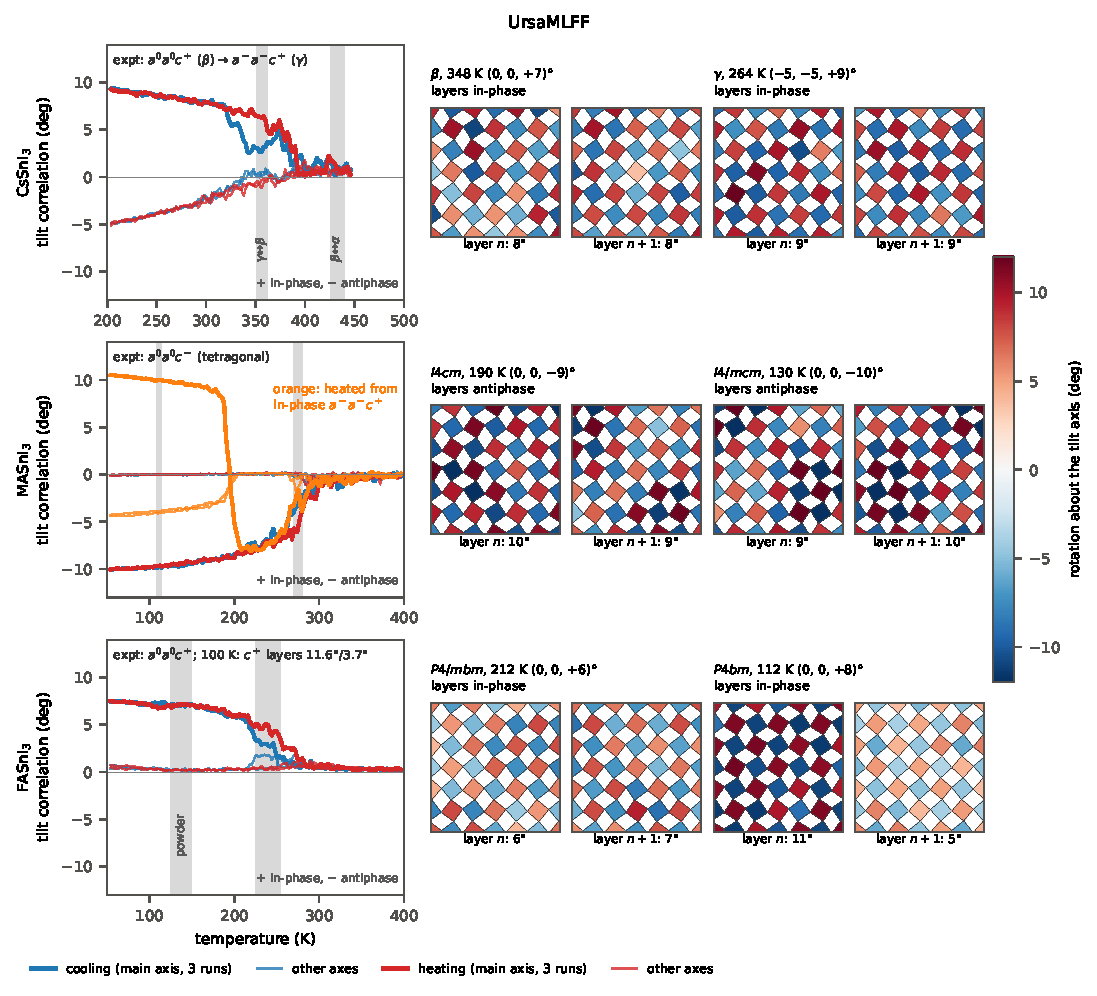
\includegraphics[width=0.74\linewidth]{wp_tiltpatterns.pdf}
  \caption{Octahedral tilts on cooling (blue) and heating (red) at \SI{0.25}{K/ps}. Left: tilt correlation of
    neighbouring octahedra about the main tilt axis (thick) and the other two axes (thin), mean of three runs; $+$
    in-phase, $-$ antiphase; grey bands: measured transitions; orange: \MASnI{} heated from an in-phase crystal. Right:
    two successive layers of octahedra in the ordered phases, each square coloured by its rotation about the tilt axis;
    in-phase stacking repeats the pattern, antiphase stacking inverts it.}
  \label{fig:wp-tilts}
\end{figure}

The simulations form the experimental tilt systems. \CsSnI{} tilts in-phase about one axis ($a^0a^0c^+$, $\beta$)
and then adds antiphase tilts about the other two ($a^-a^-c^+$, $\gamma$); \FASnI{} tilts in-phase and \MASnI{}
antiphase ($a^0a^0c^-$) in every run. The single-tilt angles agree with the measured ones to within \ang{0.3}. Below
about \SI{130}{K} \FASnI{} develops the layered tilt of its low-temperature structure, with successive layers tilted by
\ang{10.9} and \ang{4.9} at \SI{110}{K} against \ang{11.6} and \ang{3.7} measured at \SI{100}{K}. The tilt ordering of
the hybrids falls within the measured ranges, while both transitions of \CsSnI{} lie 40 to \SI{55}{K} below the
measured ones; the processing simulations below therefore place every temperature relative to the compound's own
transition.

\begin{table}[t]
  \centering\small
  \caption{Simulated (sim.) against measured (exp.) tilt systems, tilt angles and transition temperatures (heating /
    cooling). Angles: amplitude of the single tilt ($+$ in-phase, $-$ antiphase); $\gamma$-\CsSnI{}: equatorial / apical
    Sn--I--Sn bending; each compared at the same distance below its transition.\cite{Chung2012JACS,
    stoumpos2013semiconducting, Takahashi2011Dalton, Kahmann2020ACSEL, schueller2018crystal}}
  \label{tab:wp-tilts}
  \begin{tabular}{llcccc}
    \toprule
    compound & phase & tilt system & angle (deg), exp. / sim. & transition & $T$ (K), exp. / sim. \\
    \midrule
    \CsSnI{} & $\beta$ & $a^0a^0c^+$ & $+$6.0 / $+$6.2 & $\alpha\leftrightarrow\beta$ & 440, 426 / 385, 370 \\
     & $\gamma$ & $a^-a^-c^+$ & 11.3, 6.8 / 9.9, 6.7 & $\beta\leftrightarrow\gamma$ & 362, 351 / 323, 317 \\
    \MASnI{} & tetragonal & $a^0a^0c^-$ & $-$8.6 / $-$8.5 & tilt order & ${\sim}275$ / 290, 260 \\
    \FASnI{} & tetragonal & $a^0a^0c^+$ & $+$6.3 / $+$6.4 & tilt order & 225--255 / 255, 247 \\
     & low $T$ & layered $c^+$ & 11.6, 3.7 / 10.9, 4.9 & layering & 125--155 / 133, 127 \\
    \bottomrule
  \end{tabular}
\end{table}

\subsection{What sets the tilt pattern?}
\label{sec:wp-sense}
The stacking of the tilts is fixed at the first ordering transition and is inherited by the film on cooling. The
inorganic framework hardly distinguishes the two stackings, whose energies differ by about \SI{1}{meV} per formula
unit,\cite{Klarbring2019PRB} so the A-site cation must choose. We computed the free-energy difference between the
two stackings in frameworks held at the measured tilts, with only the cations moving (Figure~\ref{fig:wp-sense}b).
\FASnI{} is lower in-phase by \SI{31}{meV} per formula unit at \SI{200}{K} and by 31 to \SI{36}{meV} up to
\SI{300}{K}; \MASnI{} is lower antiphase by 15 to \SI{17}{meV}.

The cause is the shape of the cage (Figure~\ref{fig:wp-sense}a). A tilt turns each face of the cage around the
cation into a rectangle with a long axis $L$. In-phase stacking gives the lower and upper faces the same long axis;
antiphase stacking crosses them. In the in-phase cage both cations lie along the common long axis. In the crossed cage
FA, which carries an NH$_2$ group at each end and spans the cage, can follow only one face: it aligns with the far face
and lies across the near one, so one end is always squeezed (Figure~\ref{fig:wp-sense}c). MA, with a single NH$_3$
group, sits against one face and aligns with it, an arrangement that is lower in energy than in the in-phase cage.

\begin{figure}[t]
  \centering
  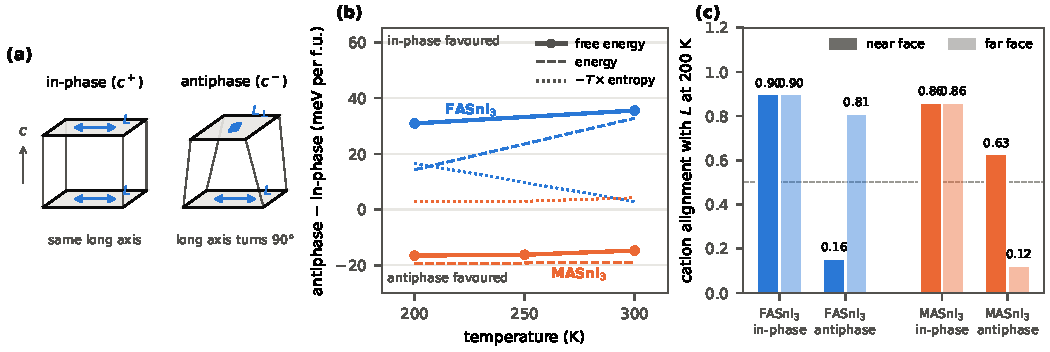
\includegraphics[width=0.9\linewidth]{wp_tilt_sense.pdf}
  \caption{Origin of the tilt stacking. (a) A tilt about $c$ makes each face of the cation cage a rectangle with long
    axis $L$; in-phase stacking keeps $L$ at the lower and upper faces, antiphase stacking turns it by \ang{90}. (b)
    Free energy of antiphase relative to in-phase stacking per formula unit, with its energy and entropy parts, in
    frameworks held at the measured tilts. (c) Alignment of the cation axis (FA N--N, MA C--N) with the long axis of the
    near and far face of its cage at \SI{200}{K}; 0.5: no preference.}
  \label{fig:wp-sense}
\end{figure}

\subsection{In which state does processing leave the film?}
\label{sec:wp-process}
With the free crystal reproduced, we add the substrate. We follow each compound through the process history of a device film: an anneal at \SI{373}{K}, cooling at
\SI{0.25}{K/ps} through the \SI{358}{K} of damp-heat testing to the operating temperature of \SI{300}{K}, and a hold
there. Each temperature is shifted by the difference between the simulated and the measured transition, so that the
film anneals and operates at the same distance from its transition as in a device. \CsSnI{} then anneals in its
$\beta$ phase and crosses into $\gamma$ during cooling, while \MASnI{} and \FASnI{} stay untilted throughout. The
substrate is described in two ways and compared with a free-standing crystal of the same history: an in-plane tension
of \SI{50}{MPa}, the measured residual stress, and an in-plane cell fixed at the end of the anneal, as for a film
bonded to a rigid substrate.

Both descriptions leave the films stretched in the plane by 0.2 to \SI{0.4}{\percent} (Table~\ref{tab:wp-film}). The
rigid substrate builds up 63 to \SI{77}{MPa}, close to the imposed \SI{50}{MPa} and to the stresses measured in
films.\cite{Rolston2018AEM, Zhao2017SciAdv, ref_processing_temp} No compound changes its tilt pattern: the constraint weakens the tilt of \CsSnI{} about the film normal from
\ang{8.5} to \ang{7.8}, and the hybrids stay untilted.

\begin{table}[t]
  \centering\small
  \caption{Processed films at the operating temperature, relative to the free crystal with the same history:
    in-plane strain $\Delta\varepsilon_\parallel$, in-plane stress $\sigma_\parallel$ (tensile positive), tilt about
    the film normal (free crystal in parentheses), and band-gap change $\Delta E_\mathrm{g}$ (mean $\pm$ standard error) of the film and of its
    purely elastic part. $^a$Preliminary.}
  \label{tab:wp-film}
  \begin{tabular}{llccccc}
    \toprule
    compound & substrate & $\Delta\varepsilon_\parallel$ (\%) & $\sigma_\parallel$ (MPa) & tilt (deg) &
      $\Delta E_\mathrm{g}$ (meV) & elastic (meV) \\
    \midrule
    \CsSnI{} & \SI{50}{MPa} tension & $+$0.40 & 50 & 8.0 (8.5) & $+$20 $\pm$ 13$^a$ & $+$18 $\pm$ 6$^a$ \\
     & rigid & $+$0.29 & 63 & 7.8 & $+$6 $\pm$ 12$^a$ & $+$19 $\pm$ 7$^a$ \\
    \MASnI{} & \SI{50}{MPa} tension & $+$0.21 & 53 & $<$1 & $+$7 $\pm$ 18 & $+$8 $\pm$ 6 \\
     & rigid & $+$0.32 & 77 & $<$1 & $+$10 $\pm$ 18 & $+$12 $\pm$ 7 \\
    \FASnI{} & \SI{50}{MPa} tension & $+$0.27 & 47 & $<$1 & $+$21 $\pm$ 20 & $+$13 $\pm$ 4 \\
     & rigid & $+$0.36 & 66 & $<$1 & $0 \pm 17$ & $+$15 $\pm$ 5 \\
    \bottomrule
  \end{tabular}
\end{table}

\subsection{Does processing shift the band gap?}
\label{sec:wp-gap}
The first device property the residual strain can change is the band gap. It was computed on snapshots of each film at the operating temperature and compared with the free crystal
(Table~\ref{tab:wp-film}). Straining free snapshots to the cell of the processed film isolates the elastic part. In
the hybrids this part opens the gap by 8 to \SI{15}{meV}; it follows the volume with a deformation potential of about
\SI{3}{eV}, as expected for a valence-band maximum of antibonding Sn 5s--I 5p character.\cite{huang2013electronic} The sign
agrees with experiment: contracting untilted FA$_{1-x}$Cs$_x$SnI$_3$ lowers its gap,\cite{Prasanna2017JACS} and in lead
halide films the more tensile surface layer emits about \SI{14}{meV} higher than the film below.\cite{Zhu2019NatCommun}
The changes of the full films agree with the elastic part, so the untilted hybrids respond elastically. At the
operating temperature the gap fluctuates by 35 to \SI{67}{meV} from snapshot to snapshot, several times the shift
caused by the process. In \CsSnI{} preliminary values give an opening of about \SI{20}{meV} under tension, again close
to the elastic part.

\subsection{Does residual strain accelerate degradation?}
\label{sec:wp-hop}
The second is the lifetime of the film. Without oxygen or moisture, the intrinsic routes of degradation are iodide migration through vacancies and, in
\CsSnI{}, conversion to the yellow phase, treated in the next section. We computed the free-energy barrier of an iodide hop into a neighbouring
vacancy at the operating temperature, with the in-plane lattice strained by $-1$, 0 and $+\SI{1}{\percent}$
(Table~\ref{tab:wp-hop}). In \CsSnI{} tension lowers both barriers, by \SI{17}{meV} per percent for hops within the
film plane and \SI{35}{meV} per percent for hops out of it; at the residual strain of a clamped film,
$+\SI{0.25}{\percent}$, iodide hops become 1.2 to 1.5 times faster. Direct simulations of cells with several
vacancies confirm the trend: at \SI{475}{K} the hop rate at $+\SI{1}{\percent}$ is $2.2 \pm 0.2$ times that of the
unstrained cell, with an activation energy of about \SI{400}{meV}. The hybrids respond less: their out-of-plane
barriers fall by 28 (\MASnI{}) and \SI{6}{meV} (\FASnI{}) per percent, their in-plane barriers are lowest under
compression, and at $+\SI{0.25}{\percent}$ their hop rates change by factors of 0.95 to 1.3. The barriers lie in the
range of measured activation energies of halide migration, $370 \pm \SI{60}{meV}$ in MASnBr$_3$\cite{Kubicki2020JACS} and
600 to \SI{680}{meV} in \ce{MAPbI3} cells.\cite{Eames2015NatCommun} Measurements on lead halide films agree in sign: the
activation energy of ion conduction in \ce{MAPbI3} films falls under tension,\cite{Zhao2017SciAdv} and tensile CsPbI$_2$Br cells degrade faster at
\SI{85}{\celsius} than compressed ones.\cite{ref_processing_temp}

\begin{figure}[t]
  \centering
  \begin{minipage}[b]{0.5\linewidth}
    \centering\small
    \captionof{table}{Free-energy barrier of an iodide hop into a vacancy (meV) against in-plane strain at the
      operating temperature; uncertainty about \SI{20}{meV}. Paths as in Figure~\ref{fig:wp-hop}.}
    \label{tab:wp-hop}
    \begin{tabular}{llccc}
      \toprule
      compound & hop & $-\SI{1}{\percent}$ & 0 & $+\SI{1}{\percent}$ \\
      \midrule
      \CsSnI{} & in-plane & 497 & 469 & 452 \\
       & out-of-plane & 409 & 373 & 338 \\
      \MASnI{} & in-plane & 333 & 392 & 397 \\
       & out-of-plane & 416 & 418 & 390 \\
      \FASnI{} & in-plane & 431 & 467 & 459 \\
       & out-of-plane & 471 & 459 & 453 \\
      \bottomrule
    \end{tabular}
  \end{minipage}\hfill
  \begin{minipage}[b]{0.46\linewidth}
    \centering
    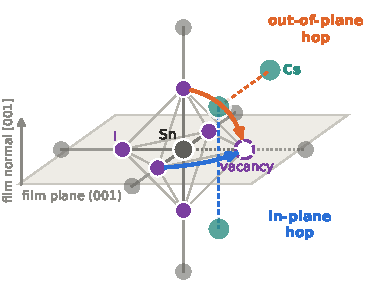
\includegraphics[width=0.78\linewidth]{wp_hop_path.pdf}
    \captionof{figure}{Iodide hop paths: from a neighbouring in-plane site or from the apical site of the same
      octahedron into an in-plane vacancy.}
    \label{fig:wp-hop}
  \end{minipage}
\end{figure}

\subsection{Can strain stabilise black \CsSnI{}?}
\label{sec:wp-yb}
Of the three compounds only \CsSnI{} has a non-perovskite competitor, a yellow phase built from chains of
edge-sharing octahedra.\cite{Chung2012JACS} Experiment fixes two points: yellow \CsSnI{} turns black only on heating,
at about \SI{425}{K}, and black films kept in air at room temperature turn yellow.\cite{Chung2012JACS,
ref_sn_instability} We computed the free energies of both phases as a function of temperature
(Figure~\ref{fig:wp-yb}). At the operating temperature the yellow phase is lower by 11 to \SI{19}{meV} per formula
unit: its lower enthalpy outweighs the larger vibrational entropy of the black phase, whose advantage grows with
temperature. The two free energies cross between 350 and \SI{385}{K}, below the \SI{425}{K} at which yellow crystals
convert on heating; the conversion rebuilds the octahedral network and sets in only above the equilibrium
temperature. The simulated yellow phase is denser by \SI{5}{\percent}, against \SI{6}{\percent} for the measured
structures,\cite{Chung2012JACS} so in-plane tension favours the black phase. The residual stress of a processed film,
50 to \SI{80}{MPa}, shifts the balance by only 2 to \SI{4}{meV} per formula unit and the crossing by 11 to
\SI{18}{K}. An in-plane strain of about \SI{1}{\percent}, the level at which substrate clamping keeps black
CsPbI$_3$ films from converting,\cite{Steele2019Science} corresponds to \SI{230}{MPa} in \CsSnI{} and moves the
crossing to 300 to \SI{335}{K}, close to the operating temperature.

\begin{figure}[t]
  \centering
  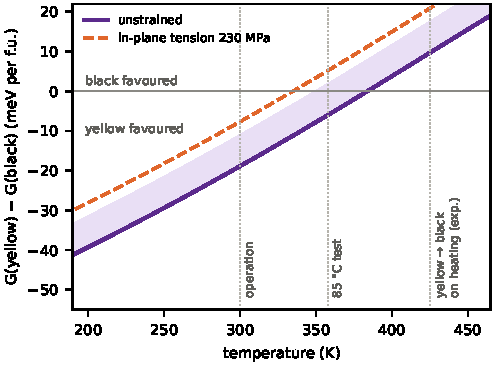
\includegraphics[width=0.48\linewidth]{wp_yb.pdf}
  \caption{Free energy of yellow relative to black \CsSnI{} per formula unit. Solid: unstrained crystal; shaded:
    uncertainty of the enthalpy difference of the two phases; dashed: in-plane tension of \SI{230}{MPa}, about
    \SI{1}{\percent} strain. Temperatures on the device scale of the processing model. Dotted: operating temperature,
    damp-heat test and the measured conversion of yellow to black on heating.\cite{Chung2012JACS}}
  \label{fig:wp-yb}
\end{figure}


\section{Discussion}
% =====================================================================================
% WHITE PAPER discussion (user 2026-11-12; restructured after a colleague's review: one question, transitions, what it
% means for experimentalists and engineers, "first step towards X"): implications, idealisations, extensions and vision.
% No functional / DFT details.
% =====================================================================================

The results trace one chain from process to device. The cation fixes the tilt pattern; the anneal and the substrate
leave the film under 0.2 to \SI{0.4}{\percent} in-plane tension, within the range measured in films, without changing
that pattern; and the tension acts more on the lifetime of the film than on its band gap. Four points follow for
experiment and manufacturing.

\paragraph{Choice of cation.} A cation with hydrogen-bonding groups at both ends (FA) selects in-phase tilting, one
anchored at a single end (MA) antiphase tilting: a criterion for anticipating the tilt pattern of new cations and
mixtures.

\paragraph{Band gap.} For the untilted hybrids the residual strain of processing shifts the gap by about \SI{10}{meV},
less than its thermal fluctuation at the operating temperature. Shifts of several tens of meV measured on such films
therefore point to causes other than processing strain, such as composition or carrier concentration.

\paragraph{Lifetime.} Residual tension speeds up iodide migration in \CsSnI{}, by 1.2 to 1.5 times at the strain left
by processing and about twice at \SI{1}{\percent}, while the hybrids are hardly affected. For \CsSnI{} films, processing
that lowers the tension should slow this route of degradation: a lower anneal temperature, a substrate or transport
layer whose thermal expansion is closer to that of the film, or a transport layer deposited hot so that it compresses
the film on cooling, as demonstrated for CsPbI$_2$Br.\cite{ref_processing_temp}

\paragraph{Black \CsSnI{}.} At the operating temperature the yellow phase is the stable one, and the residual stress of
processing shifts the balance by only 2 to \SI{4}{meV} per formula unit. Keeping a film black therefore requires
either in-plane strains near \SI{1}{\percent} or protection that keeps the conversion from nucleating.

\paragraph{Idealisations.} The simulations describe an idealised film. Each cell is a periodic single crystal a few
nanometres across, without grains, grain boundaries, free surfaces or interfaces with the transport layers, although
these relieve strain, nucleate tilt domains and offer fast paths for ions. The substrate enters only through a fixed
in-plane stress or a rigid in-plane cell; a real substrate also contracts, and the bond to the film relaxes over hours,
so the rigid case is an upper bound of the residual strain. The films are cooled many orders of magnitude faster than in
processing, and slow, reconstructive changes such as the conversion of black to yellow \CsSnI{} are treated through
free energies rather than followed directly. The chemistry is
restricted to the perovskite and its cation and iodide vacancies: oxygen, moisture, the oxidation of Sn(II) to Sn(IV),
light and excess charge carriers, which drive the degradation of tin films in practice,\cite{ref_sn_instability} are
not included.

\paragraph{Extensions and vision.} These idealisations can be removed step by step. Adding oxygen and nitrogen will
compare processing and operation in air with inert nitrogen atmospheres and give access to the first steps of Sn(II)
oxidation. Polycrystalline cells with grain boundaries, built from cells of tens of thousands of atoms that already
form tilt domains, will show how boundaries relieve the residual strain, pin the tilt variant that forms on cooling
and channel iodide migration. An explicit substrate and transport layer will replace the idealised boundary
conditions by the real interface and its mismatch of thermal expansion. This white paper is the first step toward a
virtual process line for perovskite absorbers. With these extensions the same framework can rank process windows
(anneal temperature, cooling rate, substrate, transport layer and atmosphere) by the band gap and lifetime they
produce, and test compositions before they are synthesised. For manufacturers this replaces part of the trial and
error of process tuning by a screened search; for experimentalists it provides the structural picture needed to
interpret diffraction, photoluminescence and ion-migration measurements on strained films.


% bibliography style set by the achemso package (a second \bibliographystyle breaks BibTeX)
\bibliography{JCTC}

\end{document}
